\section{Theorie}
\label{sec:Theorie}

Wird Licht als eine Wele angenommen, so können Beugungseffekte von Licht an einem Spalt erklärt werden. Nach dem Huygensschen
Prinzip ist jeder Punkt an einer Wellenfront der Ausgangspunkt einer Elementarwelle. Die Elemtentarwellen interferieren miteinander
und erzeugen eine neue Wellenfront. In diesem Versuch wird nur die Fraunhofer Beugung (siehe Abbildung 1) betrachtet, da diese
mathematisch einfacher zu behandeln ist. Anders als bei der Fresnel Beugung wird bei der Fraunhofer Beugung ein
paralleler Strahlengang von einer weit entfernten Lichtquelle vorrausgesetzt.


\begin{figure}[H]
  \centering
  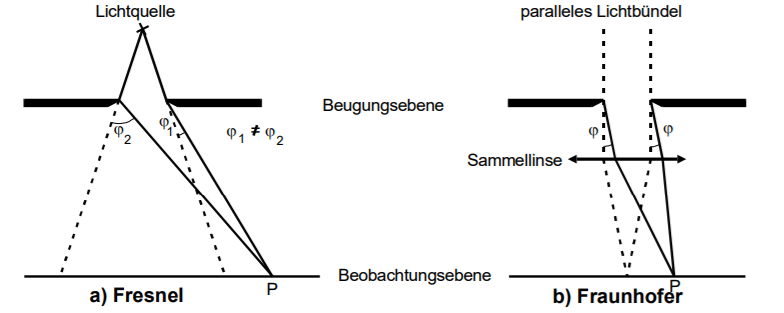
\includegraphics[height=5cm]{fraunhofer.PNG}
  \caption{Darstellung von Fresnel und Fraunhofer Beugung \cite{sample}.}
  \label{fig:biegungbild1}
\end{figure}

Fällt nun eine ebene Welle $A(z, t) = A_0 exp(i(\omega t -2\pi z/\lambda))$ ein, errechnet sich der Schwingungszustand  eines
beliebigen Punktes in dem Wellenfeld durch Überlagerung aller Elementarwellen die zur gleichen Zeit an dem Punkt ankommen. Hierbei bezeichnet
$\lambda$ die Wellenlänge, $t$ die Zeit und $z$ die Richtung.
Für zwei Strahlbündel im Abstand $x$ ergibt sich, ausgehend von dem Spalt, eine Phasendifferenz von
\begin{align}
  \delta = \frac{2\pi s}{\lambda} = \frac{2\pi x \sin{\varphi}}{\lambda}
\end{align}

Für die Amplitude $B$ in einer Richtung $\varphi$ muss über alle in diese Richtung gebeugte Strahlenbündel summiert werden. Es ergibt sich:
\begin{align}
  B(z,t, \varphi) = A_0 e^{i \left(\omega t - \frac{2\pi z}{\lambda} \right)} e^{\frac{\pi i b \sin{\varphi}}{\lambda}} \frac{\lambda}{\pi \sin{\varphi}}
  \sin{\left(\frac{\pi b \sin{\varphi}}{\lambda}\right)}
\end{align}

Dabei sind $b$, $s$ und $\varphi$ wie in Abbildung 2 definiert.

\begin{figure}[H]
  \centering
  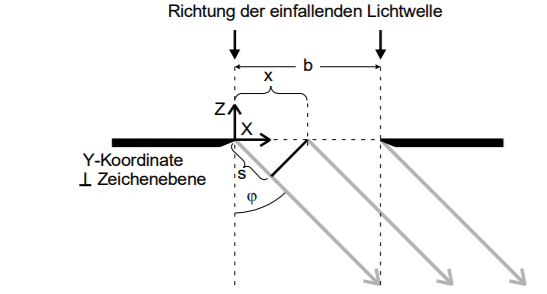
\includegraphics[height=5cm]{beugung.PNG}
  \caption{Phasenbeziehung zwischen Strahlenbündel \cite{sample}.}
  \label{fig:biegungbild1}
\end{figure}



Für die Intensität des am Spalt gebeugten Lichts gitl:
\begin{align}
  I(\varphi) \propto B(\varphi)^2 = A_0^2 b^2 \left(\frac{\lambda}{\pi b \sin{\varphi}} \right)^2  \sin^2{\left(\frac{\pi b \sin{\varphi}}{\lambda}\right)}
\end{align}

Die durch Gleichung (3) beschriebene Funktion wird als Beugungsfigur bezeichnet.

Die Intensitätsverteilung des Doppelspaltes setzt sich aus den Intensitätsverteilungen des Einzelspaltes zusammen.
\begin{align}
   I(\varphi) \propto B(\varphi)^2 = 4 \cos{\left(\frac{\pi s \sin{\varphi}}{\lambda}\right)} \left(\frac{\lambda}{\pi b \sin{\varphi}}\right)^2
   \sin^2{\left(\frac{\pi b \sin{\varphi}}{\lambda}\right)}
\end{align}
